\chapter{Theoretical Framework: Complexity and Efficiency}\label{chapt:2}

\section{Computational Complexity}

Computational complexity refers to the study of the resource requirements of algorithms, primarily focusing on time and space resources as functions of the input size. This field categorizes problems based on the minimal resources needed for solving them, providing a theoretical framework for understanding the intrinsic difficulty of computational problems and the efficiency of algorithms designed to solve them. ~\cite{GareyJohnson1979}

\subsection{Time Complexity}

Time complexity is a measure of the amount of computational time that an algorithm takes to complete as a function of the length of the input. It is often expressed using Big O notation, which describes the upper bound of the growth rate of the runtime~\cite{BigONotation}. Understanding an algorithm's time complexity is crucial for predicting its scalability and feasibility in practical applications, especially for problems known to be computationally intensive, like the Travelling Salesman Problem (TSP).

The TSP, being NP-hard, does not have a known polynomial-time solution that can solve all instances of the problem efficiently. The brute-force approach to TSP, for instance, has a factorial time complexity (\(O(n!)\)), making it computationally infeasible for even moderately sized problem instances. This has led to the exploration of various heuristic and metaheuristic algorithms that aim for acceptable solutions in polynomial time (\(O(n^k)\)), where \(k\) is a constant, trading off exactness for efficiency and practical applicability.~\cite{Dorigo1996}

\begin{figure}[h]
	\centering
	\caption{Growth rate of different complexities}
	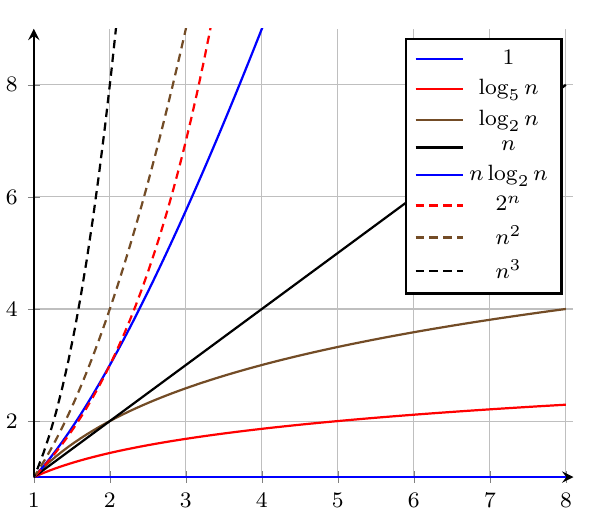
\begin{tikzpicture}
		\begin{axis}
			[
				axis lines = left,
				xmin=1, xmax=8.1, ymin=1, ymax=9,
				domain=0:8, samples=100, no markers, thick, grid=both,
				xlabel = \(n\), ylabel = {\(f(n)\)},
				label style = {overlay},       % Has he same effect as
				ticklabel style = {overlay},   % trim axis [left|right]
				legend entries = {
						$1$,
						$\log_{5}n$,
						$\log_{2}n$,
						$n$,
						$n\log_{2}n$,
						$2^{n}$,
						$n^{2}$,
						$n^{3}$,
					},
				every axis/.style = {font=\footnotesize},
				label style = {font=\normalsize},
			]
			\addplot+ {1};
			\addplot+ {1 + ln(x)/ln(5)};
			\addplot+ {1 + ln(x)/ln(2)};
			\addplot+ {x};
			\addplot+ {1 + x*ln(x)/ln(2)};
			\addplot+ {2^x-1};
			\addplot+ {x^2};
			\addplot+ {x^3};
		\end{axis}
	\end{tikzpicture}
\end{figure}

\subsection{Space Complexity}

Space complexity measures the total amount of memory an algorithm needs to run to completion as a function of the input size. Like time complexity, space complexity is crucial for evaluating an algorithm's efficiency, particularly in scenarios where memory resources are limited. In the context of the TSP and similar optimization problems, the space complexity of an algorithm can significantly impact its usability in real-world applications, where solutions often need to be computed on-the-fly or on hardware with constrained memory capacities.~\cite{HeldKarp1962}.

For example, dynamic programming approaches to the TSP, such as the Held-Karp algorithm, offer a more favorable time complexity compared to brute force (\(O(n^2 2^n)\)) but at the cost of exponential space complexity (\(O(n^2)\)). Such trade-offs between time and space complexity are central considerations in algorithm design, especially when developing new algorithms intended for large-scale problem instances, like those encountered in logistics and routing applications.


\section{P vs. NP Problem}

The P vs. NP problem is one of the most fundamental unsolved questions in computer science. It asks whether every problem whose solution can be quickly verified (in polynomial time) by a computer can also be quickly solved (in polynomial time) by a computer. The class P consists of problems that can be solved quickly, while the class NP consists of problems for which a proposed solution can be quickly checked.~\cite{PvsNP}.

\subsection{Definition and Significance}

Formally, a problem is in the class P if it can be solved in polynomial time, meaning the amount of time to solve the problem grows polynomially with the size of the input. The class NP, on the other hand, encompasses problems for which any given solution can be verified in polynomial time. The P vs. NP question essentially asks if these two classes are the same; that is, if every problem that can be verified quickly can also be solved quickly.

The significance of the P vs. NP problem lies in its implications for a vast range of disciplines, from cryptography and algorithm design to decision-making processes and beyond. A proof that P equals NP could potentially revolutionize the fields of mathematics and computer science, enabling efficient solutions to a multitude of complex problems currently considered intractable. Conversely, proving that P does not equal NP would formalize the intrinsic computational hardness of these problems.

\subsection{Implications for TSP}

The classification of the Travelling Salesman Problem (TSP) as NP-hard underscores the complexity and computational challenges associated with finding an exact solution for large instances of the problem. This categorization has significant implications for both theoretical research and practical applications in the field. It implies that unless P equals NP—a question that remains one of the most fundamental unsolved problems in computer science—we should not expect to discover an algorithm that can solve every instance of TSP quickly (in polynomial time) and accurately. This realization has shifted the focus of much of the research on TSP towards the development of heuristic and metaheuristic algorithms, which aim to find good-enough solutions within a reasonable timeframe, rather than pursuing the elusive goal of an exact solution for all possible instances.~\cite{Karp1972}.

Furthermore, the implications of TSP being NP-hard extend beyond algorithm development. It influences how problems are modeled in practical scenarios where TSP-like problems arise, such as logistics and routing, network design, and scheduling. In these applications, the emphasis is often on finding solutions that are close to optimal but can be obtained much more quickly than what an exact algorithm would allow. This approach allows industries to achieve efficiency and cost savings even when dealing with complex routing and scheduling problems.

Additionally, the study of TSP and its place within the NP-hard class has spurred interest in exploring the limits of computational power and understanding the inherent difficulty of various computational problems. It challenges researchers to continually innovate and find new ways of approaching problem-solving in computational mathematics and computer science. As such, the implications of TSP's classification resonate through both the academic study of algorithm theory and the practical considerations of applying these theories in real-world situations.


\section{Complexity of TSP}

The proof that the TSP is NP-hard was first presented by Richard M. Karp in 1972. Karp's work, part of a seminal paper that identified 21 NP-complete problems, laid the groundwork for understanding the computational limits of algorithmic solutions to TSP and similar problems. By demonstrating that the decision version of the TSP (determining whether there exists a tour of a given length or less) is NP-complete, Karp effectively showed that the optimization version of TSP, where the goal is to find the shortest possible tour, is NP-hard.

Karp's proof employs a technique known as reduction, whereby a known NP-complete problem is transformed into an instance of the TSP in polynomial time. This method illustrates that if a polynomial-time algorithm could solve TSP, it could, by extension, solve all problems in NP, a proposition that remains unverified. Thus, the proof not only marks the TSP as a fundamentally challenging problem but also deepens our understanding of the landscape of computational complexity.

The implications of TSP's NP-hardness are far-reaching in the realm of algorithm design. It signals that, unless P=NP, there is no algorithm that can solve all instances of the TSP efficiently. This realization has spurred the development of various heuristic and approximation algorithms, which aim for practically good, though not always optimal, solutions within reasonable computational time frames.

\subsection{Impact on Algorithm Design}

The NP-hardness of TSP has a profound impact on how algorithms for solving it are designed, fostering the development of various strategies that aim to circumvent the computational hurdles:

\begin{itemize}
	\item \textbf{Exact Algorithms:} Despite the NP-hardness of TSP, exact algorithms, such as the Held-Karp algorithm, have been devised. These algorithms guarantee an optimal solution but do so at a computational cost that increases exponentially with the problem size, rendering them impractical for large instances.
	\item \textbf{Heuristic Approaches:} To tackle larger instances of TSP, heuristic algorithms are employed. These algorithms do not guarantee an optimal solution but can often find good solutions in a fraction of the time required by exact methods. Examples include the Nearest Neighbor and Christofides' algorithm.
	\item \textbf{Metaheuristic Algorithms:} For even more complex instances, metaheuristic approaches, like Genetic Algorithms and Ant Colony Optimization, offer flexible strategies that explore the solution space more broadly, aiming to escape local optima and approach global optima more effectively. These techniques draw inspiration from natural processes and have the advantage of adaptability to different problem instances.
	\item \textbf{Approximation Algorithms:} Given the NP-hardness of TSP, approximation algorithms that provide provable guarantees about the closeness of the solution to the optimum are particularly valuable. These algorithms are especially pertinent for specific variants of TSP, like the Metric TSP, where they can leverage the triangle inequality to bound the solution quality.
\end{itemize}

The NP-hardness of TSP thus not only underscores the intrinsic difficulty of the problem but also catalyzes innovation in algorithm design, pushing the boundaries of what can be computationally achieved within the constraints of computational complexity.


